\subsection{Modell} \label{subsec:modell}

Für die Berechnung der potentiellen Energie benützen wir das Modell Park Avenue 432, eines der höchsten reinen Wohnhochhäusern auf der Welt. Die stolze Höhe und der über das ganze Gebäude gleichbleibende quadratische Grundriss sind ideal für unsere Berechnungen. Für die Wassermengenberechnung stützen wir uns auf die Angaben des durchschnittlichen Wasserverbrauch in Amerika pro Person und Tag: 314\si{L}. \cite{waterUsAmerica}

\begin{figure} [H]
	\centering
	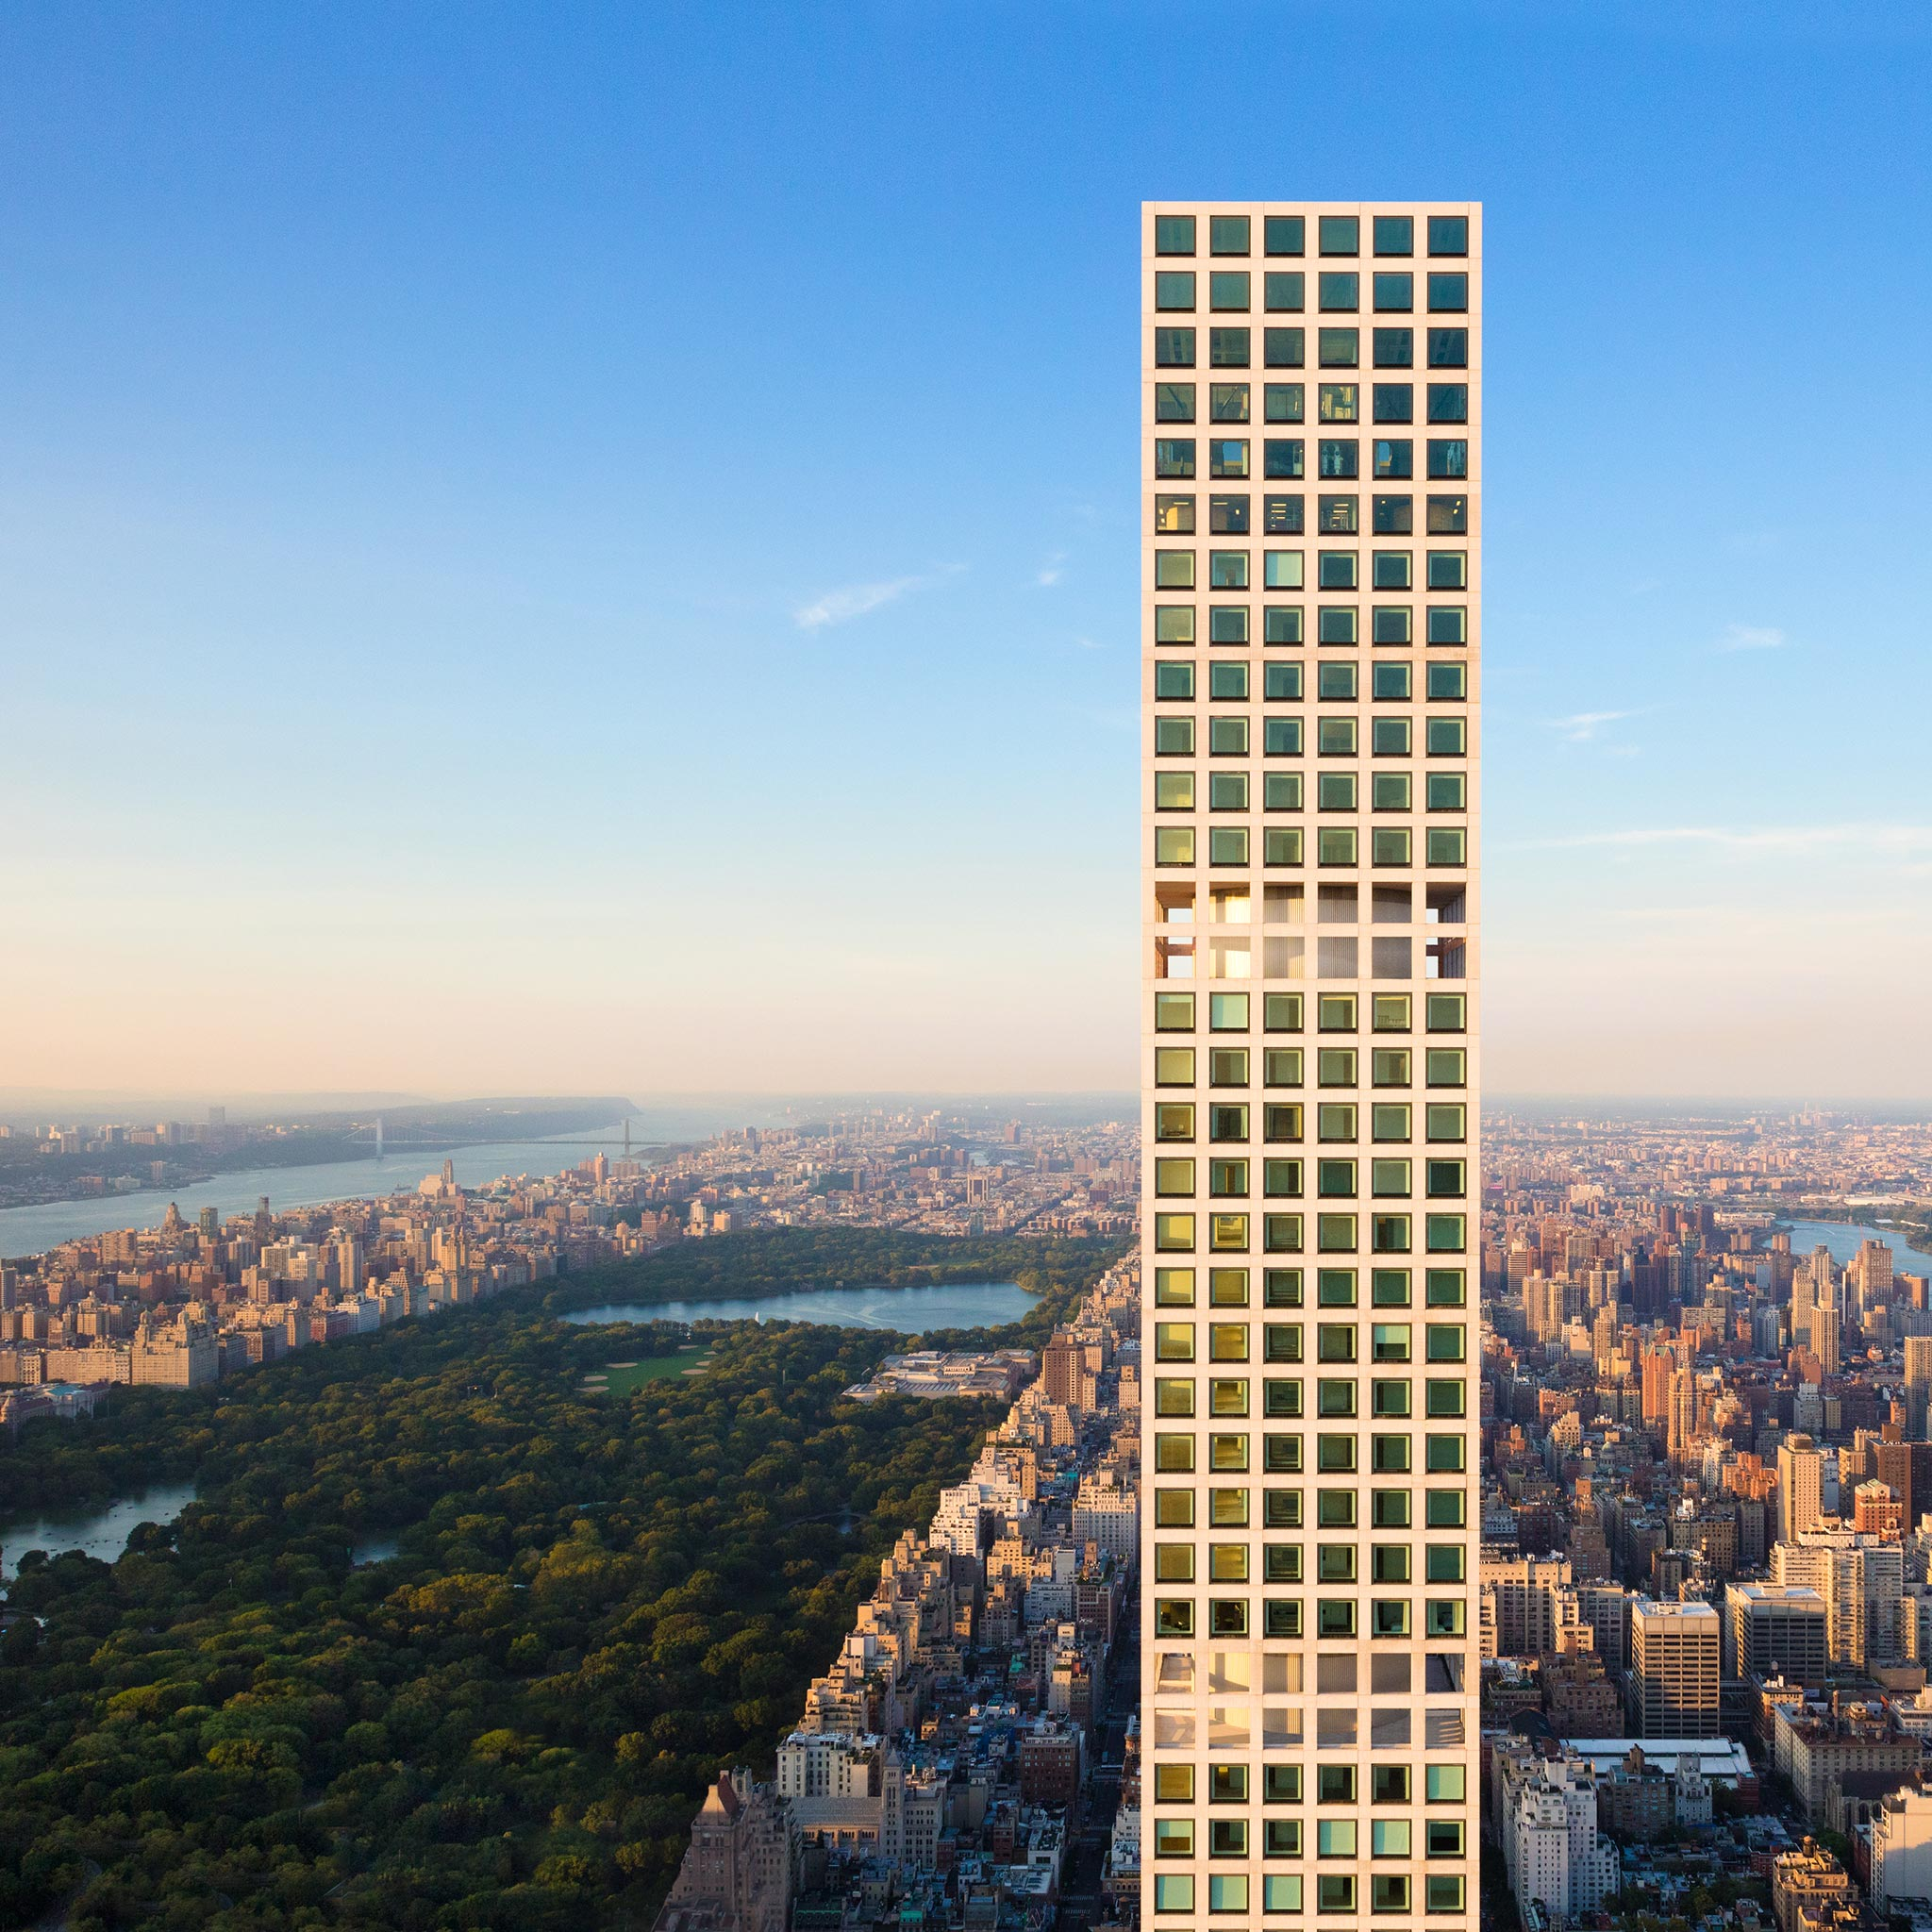
\includegraphics[width=12cm]{parkAvenue.jpg}
	\caption{Park Avenue 432 \cite{432_Park_Avenue}}
	\label{fig:Park_Avenue_432}
\end{figure}

\begin{table}[H]
\centering
\begin{tabular}{ll}
Name:				&Park Avenue 432\\
Höhe: 				&426m\\          
Etagen:				&84 Obergeschosse, 1 Erdgeschosse, 3 Untergeschosse\\
Etagenhöhe:			&4.72m\\
Hoechste Etage:		&392.1m\\
Wohnungen:			&104\\
Speziell:			&alle 12 Etagen 2 Etagen leer\\           
\end{tabular}
\end{table}

\newpage
